\documentclass[conference]{IEEEtran}
\IEEEoverridecommandlockouts
% The preceding line is only needed to identify funding in the first footnote. If that is unneeded, please comment it out.
\usepackage{cite}
\usepackage{amsmath,amssymb,amsfonts}
\usepackage{algorithmic}
\usepackage{graphicx}
\usepackage{textcomp}
\usepackage{xcolor}
\usepackage{alltt}
\usepackage{multicol}

\def\BibTeX{{\rm B\kern-.05em{\sc i\kern-.025em b}\kern-.08em
    T\kern-.1667em\lower.7ex\hbox{E}\kern-.125emX}}
\begin{document}
\title{Process Comparisons Between the Raspberry Pi's CPU and GPU\\}

\author{\IEEEauthorblockN{1\textsuperscript{st} Ethan Moore}
\IEEEauthorblockA{\textit{School of Engineering and Applied Sciences} \\
\textit{Western Kentucky University}\\
Bowling Green, United States \\
ethan.moore416@topper.wku.edu}
\and
\IEEEauthorblockN{2\textsuperscript{nd} Zachary Mers}
\IEEEauthorblockA{\textit{School of Engineering and Applied Sciences} \\
\textit{Western Kentucky University}\\
Bowling Green, United States \\
zachary.mers@gmail.com}
}

\maketitle


\begin{abstract}
In this paper, we used the GPU and CPU of a Canakit Raspberry Pi 3 to test their efficiency compared to one another. We performed two experiments to test this. The first of these experiments was a pencil drawing experiment, in which we checked the speed at which the GPU and CPU were each able to process the images they were provided. The second experiment was processing a video for anomalies, during which each component was once again monitored for its speed.\\
For the first experiment, we found that the RPi CPU was faster than the GPU. The margin between them, however, quickly dropped with larger image sizes. Where the CPU was over sixteen times faster with the first set of images, this quickly dropped to eight times faster with the third. While GPU times being longer than the CPU equivalent was unexpected, this does support GPUs becoming more effective with larger graphical processes, a result which is consistent with prior works in this area. \\
In the second experiment, we found very similar results. The GPU was much slower than the CPU, and yet once again it showed a trend indicating that, given a sufficiently large and complex input, the GPU would eventually outpace the CPU. In its case, the minimum percent increase in average processing time for the CPU was almost double the GPU's maximum.
\end{abstract}

\section{Introduction}
Due to their different designs, GPU's and CPU's vary heavily on what they can accomplish. For example, GPU's are "often used when real-time performance in video processing is required"\cite{Blair}. They are broadly most valuable in these sorts of situations, where their ability to run a much larger number of tasks in parallel compared to their CPU counterparts allows them to quickly tackle large and complex problems. Instances of this include the topic of Fast 2-D Ultrasound Strain Imaging, which found that when it came to its namesake "using OpenMP or a GPU significantly reduces the computation time."\cite{Idzenga} Other works referenced in this paper generally came to similar conclusions, with the GPU being effective at everything from creating pencil-styled art out of photos to transferring medical data. This increase in computation time then leads into further benefits. In some cases, the increase of speed can even overcome power consumption, allowing the GPU to effectively "reduce energy consumption by as much
as 272 times" in Rakvic's paper "Energy Efficient Iris Recognition With Graphics Processing Units"\cite{Rakvic}. However, GPUs are not universally better. As an example, Jiménez found in Implementation of RSA Signatures on GPU and CPU Architectures that "in spite of its massive parallelism, we observe that GPU implementations of RSA are considerably slower than their CPU counterparts"\cite{Jimenez}. Whether GPUs or CPUs are preferable depends heavily on the task at hand, and especially on the amount of data that task will involve.\\
As stated prior, much of the reasoning for this is the GPU's ability to operate tasks in parallel. As Rakvic put it, "the number of CPU cores is in the single digits, while the number of GPU cores is approaching thousands"\cite{Rakvic}. Where a CPU must complete its task one part at a time, the GPU can do hundreds of parts at once. The reason this sometimes falters is that an individual GPU core is often weaker than one for a CPU, meaning each individual segment of the process is slower. If most steps in that process rely on those before them, a CPU will usually outperform an equivalent GPU.\\
While beginning our project, we believed the gray scale image processing experiment could potentially highlight the GPU's lead over the CPU's processing technique. The real-time anomaly detection process also could potentially show the GPU's strength by being able to more effectively work with incoming data. The original fast pencil drawing generation experiment used an in-house algorithm of their own design. Our experiment primarily utilized OpenCV's convert color method. The high resolution gray-scale images will look similar to the generated pencil drawing without the need for our own complex algorithm. While this image processing technique is not identical, it still follows the general theme of utilizing the GPU's processing technique for image creation. The image resolutions in the Parallel Fast Pencil Drawing Generation Algorithm had "test set of this experiment: 1024×768, 1280×960, 1440×1080, 1920×1440, and 2560×1920"\cite{Liu}. In our experiment we used several similar test sets, each with a different resolution. These resolutions were originally planned to be 1280x720, 1920x1080, 2560x1440, 3840x2160, and 7680x4320, but technical issues forced the largest two sets to be dropped. \\
Another difference in experiments is our GPU. In Qiu's experiment he used "two NVIDIA Tesla P100 GPUs." whereas we used the Raspberry Pi 3's Broadcom RPi GPU\cite{Liu}. Qiu found in his experiment that "the experimental results demonstrate that the parallel pencil drawing generation algorithm achieves an average acceleration of 448.59 times on 2560×1920 -resolution images and the grayscale histogram is very close to the true pencil drawing", whereas we could not expect the same results due to our different and often weaker hardware.\cite{Liu}. Nonetheless, these results still provided a rough guideline for our anticipated results in gray-scaling high resolution images.\\
As for the real-time anomaly detection experiment, our source utilized a modified OpenCV, whereas we instead used the stock OpenCV package. Our focus in detecting anomalies was not on parked cars or on pedestrians but various random objects. We did not implement different prioritization methods in favor of having one test for the CPU and GPU, which would study the RPi primarily in terms of its speed. Additionally, in Blair and Robertson's paper "these priorities dynamically change with scene content"\cite{Blair}. Our anomaly detection experiment did not attempt this priority changing implementation. These factors combined allowed us to make a far simpler program, while still thoroughly testing the RPi's CPU and GPU. As a result, we expected to obtain similar results to Blair and Robertson, who found that GPUs "can allow greater numerical precision due to their native reliance on floating-point arithmetic, but draw considerably more power"\cite{Blair}.\\
Our initial expectations were that the GPU would rapidly outpace the CPU in both experiments, as it had on other platforms in prior experiments. In addition, we expected that the degree to which it would do so would increase with more complex tasks. This was heavily based upon the results found in Qiu's Pencil Drawing program, in which similar results had been found. These expectations were proven partially wrong, however. We found instead that the GPU is the weaker of the two for the subjects of our first experiment, but that the trend of the GPU growing more effective with task size would hold. Our second experiment backed up these results, once again finding the RPi CPU to be much stronger than its GPU counterpart. It also found a repetition of the trend, with the GPU's maximum processing time increase still being merely half of the CPU's minimum. 

%\begin{table}[h]
%\begin{tabular}{|l|l|l|}
%\hline
%header 1 & Header 2 & Header 3 \\ \hline
%         &          &          \\ \hline
%         &          &          \\ \hline
%         &          &          \\ \hline
%\end{tabular}
%\end{table}

%more text..  Take a look at figure.


\section{Related Work}
Similar work can be found in "A Taste of Scientific Computing on the GPU-Accelerated Edge Device", written by Pilsung Kang and Sungmin Lim. This paper tested several GPUs and one CPU against one another, acting to compare their abilities when it came to scientific computing. It found that the Jetson Nano specifically performed well compared to its counterparts, although it had some issues in tasks requiring high memory (even failing outright during one). While the tested CPU did perform better than the non-Nano GPUs in some tests, its performance in others was the worst of every device tested. At times, "the performance gap between Jetson Nano and the AMD desktop" was as high as 60 times better for the Nano compared to the AMD CPU.\cite{Kang}. Notably, this shows that GPUs are not universally better than an equivalent CPU, something further proven by our own results. Whether the GPU or CPU is more effective is situational, and is usually determined by factors such as task complexity.\\
In Tang's paper "CPU–GPU Utilization Aware Energy-Efficient Scheduling Algorithm on Heterogeneous Computing Systems" the focus shifted from scientific computing to the CPU-GPU role of being resourceful and environmentally conscious. Tang states that "One of the main challenges for such infrastructure is energy consumption, which generates high operational costs and produces a dramatic increase in carbon."\cite{Tang}. Their approach in dealing with "the optimal CPU-GPU utilization and job deadline scheduling constraint" achieved great results\cite{Tang}. For example, "H-PSO is better than UEJS by 36.5\%, Max-EAMin by 36.3\%, and GA by 46.7\% in term of the job average energy consumption for heterogeneous system with high workload."\cite{Tang}.\\
In "Scheduling Challenges and Opportunities in Integrated CPU+GPU processors," the CPU and GPU are similarly compared with the goal of determining which can be used more efficiently for various processes. The end result was power scheduling which "outperforms the application-based and state-of-the-art scheduling methods by 40\% and 31\%, respectively.", while providing " up to 10\% more energy saving"\cite{Dev}. This is achieved by determining whether GPU or CPU is more suited for each task, based on measures such as power consumption and runtime. This bears similarity to our own experiments, which used the same metric to determine each subject's efficiency.\\
The paper "Multi-GPU Implementation of Nearest-Regularized Subspace Classifier for Hyperspectral Image Classification" mentions that "In the early remote sensing processing oriented parallel accelerations, the CPU parallel technologies dominated the primary studies"\cite{Ni}. The use of CPU parallelization was the standard in the beginning of remote sensing studies, however, this has changed. Further in the paper it states that the "GPU has become a universal computing platform for many data-intensive and computing-intensive scenarios. Compared to traditional CPU parallelism, it can achieve a dozen to several hundred times of acceleration."\cite{Ni}. Instead of using just one GPU for computation their was also a multi-GPU comparison. The results explain that "the algorithms based on single GPU accelerate by 0.28× at least and 12.85× at most, and the algorithms based on multi-GPUs accelerate by 1.3× at least and 50.57× at most."\cite{Ni}. The greater increase in performance by utilizing multiple GPU's could be a consideration when one GPU is not fast enough.\\
"GPU-Oriented Architecture for an End-to-End Image/Video Codec Based on JPEG2000" also bore similarity to our experiments, particularly our video-processing experiment. It utilized a GPU to compress high-quality video in real time, providing much more effective results than a CPU alternative. Specifically, their approach "yields results at least 10× superior on average to those achieved with JPEG2000 implementations devised for CPUs" when the subject was a 12k video\cite{Cea-Dominguez}. This is very similar to and thus an excellent comparison point for both our pencil drawing and video processing experiments, which were focused on the same topic. We were able to use their data as a rough guide for what our own should look like, acting as an extra barrier against an error in our experiments skewing the results.\\
In "Parallel and High Speed Hashing in GPU for Telemedicine Applications" the authors focus on the use of the GPU to quickly and effectively provide remote medical care. Using a CPU for this task would require either significantly weakened security or a potentially life-threatening slowdown of data. The solution presented was to instead utilize the GPU, which can handle the large amounts of medical data without a loss of security for their contents. The technique used in the paper implemented "LI tree-mode Keccak hash function in GPU" and also "demonstrated that one thread hashing one copy of Keccak is the best parallel granularity in GPU."\cite{Lee} The reason one thread was used is because of the need to use shared memory. Having more threads necessitated the increased sharing of "intermediate state and variables, hence increasing the memory read/write operations."\cite{Lee} The conclusion found was that when it came to larger and more complex tasks such as the secure transfer of medical data, the GPU was preferable to the CPU. This reinforced the idea that the GPU would increasingly grow more effective in comparison to the CPU, a finding we would replicate ourselves.\\
"Fast 2-D Ultrasound Strain Imaging: The Benefits of Using a GPU" also focused on the medical field, and as its name suggests was specifically based upon the use of a GPU when it came to 2D ultrasounds. Ultrasounds are used in the medical field to detect health conditions such as cancer, but are frequently divided into two categories: those which take hours to process, and those that operate in real time with significant errors. Both of these are less than ideal in the time-sensitive and precise work in the field. Using a GPU, however, "significantly reduces the required computation time and increases the frame rate for motion estimation", allowing it to operate quickly without sacrificing accuracy. This is in large part because of a GPU's ability to operate more effectively in parallel. Where a CPU has to complete each step of the ultrasound in order, a GPU can run several steps at once to massively increase efficiency.\\
"Optimized Real-Time MUSIC Algorithm With CPU-GPU Architecture" found another example of a GPU aiding with a highly complicated task. It focused on the Multiple Signal Classification algorithm, or MUSIC. This algorithm is used in various fields to estimate the sources of signals, but is highly resource-intensive. This severely limits its ability to be used in real-time with a conventional system. Cue the use of a GPU. Several studies "are dedicated to accelerating MUSIC algorithm by parallel hardware, especially by Graphics Processing Units (GPU)"\cite{Huang}. Like many others, this paper is focused primarily on using the CPU and GPU in parallel. The GPU is used to its specific strengths, and those strengths are highlighted for their significant impact on performance. For example, Huang found that "the parallel optimization of peak search via the GPU saves the transmission time of SPS and accelerates the entire process"\cite{Huang}. Additonally, "the GPU-Config5 strategy was shown to have performance benefits of 150x to 160x in comparison to the CPU-Config1 strategy," once again showing the massive difference between the CPU and GPU when one is in its ideal conditions\cite{Huang}. Huang's work is also another example of what those conditions are. A GPU is best for a complex task in which multiple parts can be done in parallel, such as processing the data from the MUSIC algorithm.\\
The paper "nnAudio: An on-the-Fly GPU Audio to Spectrogram Conversion Toolbox Using 1D Convolutional Neural Networks" had great success in GPU utilization. Their solution to increase audio processing needed to "dynamically train the kernels (including Fourier kernels, Mel filter banks, and CQT kernels) as part of the larger neural network training" \cite{Cheuk}. This process of training kernel code "significantly reduces the computation time from 983 minutes to only 99 minutes." \cite{Cheuk}. In our experiments we did not implement a neural network to optimize kernel code, however, the addition of neural network optimization could have possibly improved results. The kernel code we utilized for experiment 1 was incredibly basic so dramatic improvement is unlikely. The more complex math for experiment 2 could be further optimized since it needed more computation.\\
Finally, "Parallel Fast Pencil Drawing Generation Algorithm Based on GPU" also bear a large number of similarities, which is what prompted our use of its subject as one of our own experiments. This paper attempted to use the GPU to increase the speed of processing an image to resemble a hand-drawn sketch by pencil. While its chief focus was on using the GPU and CPU in parallel, both CPU and GPU variants of their program were tested. It found that CPU processing time rose quickly alongside image size, while GPU time remained mostly the same regardless. In addition, time-cost for CPU was incredibly high in comparison to GPU and the parallel program, surpassing its GPU counterpart 100 times over in some tests As with the prior work, this backed many of our initial ideas on what our results would look like, and aided in interpreting what we found.

\section{Experiment 1}
Both of our experiments were tested on a Raspberry Pi 3. Our original plan was to use the RPi4, but at the time of writing this does not appear to be supported by OpenCL. As OpenCL proved to be necessary to access the GPU for the sake of our experiments, this forced us to instead utilize the previous RPi model. Thankfully, it has much greater support, and we were able to proceed from there.\\
Our first experiment was to flip an image from color to grayscale, emulating a pencil drawing program from Qiu's similar experiment. Our variation on this was to convert each image to a black-and-white image. While this is a much simpler task than the original experiment, it requires a much lower amount of complex code. This therefore the chance that our programming could accidentally be made to favor the CPU or GPU in a way not accounted for by the experiment, while still acting as a measurement of each piece of hardware. Our expectation was that the GPU would outperform the CPU, and would be comparatively more effective with larger images. While the former did not occur in our tests, the latter did.

\subsection{Methodology}
Our original experiment's methodology for using the GPU to create pencil-like drawings stemmed from using the Raspberry Pi 4's Broadcom Videocore VI. We had planned to use the Github repository Py-Videocore6 and utilize the QPU's power due to our familiarity with Python compared to C++ and the repository's support for the Videocore VI architecture. However, several issues arose from the lack of documentation on the project. Our revised approach was to use the older Raspberry Pi 3 instead of the Pi 4 and use the Py-Videocore repository instead of the originally-planned Github repository, as it was much more effective and had far greater support on the older platform. This did introduce a potential problem in that the kernel code within the program executed has access to any part of the main memory. Running the scripts with OpenCL therefore must require root access. While we were not particularly concerned, as our Pi was adequately secure and lacked any critical information stored on it, it could be relevant in similar experiments in the future.\\
In our second setup of the experiment, the Videocore VI QPUs (Quad Processing Units) took in the multi dimensional array of values which represented the rows of pixels. Each pixel contained three values that represented blue, green, and red. Every pixel value needed to be multiplied by the corresponding decimal value and then added together to get the grayscaled value for that pixel. OpenCV's documentation lists the formula RGB[A] to Gray: Y←0.299 * R + 0.587 * G + 0.114 * B for converting BGR pixel values to their luminous counterparts. The computation required was the ability to multiply and add arrays of values. The specific implementation of OpenCL doing the computation is within our gpuOperation method. The method gpuOperation starts by finding the devices that can perform computation like the CPU and in our case the GPU. Instantiating the context, sources, and kernel codes. The program is then built and then buffers are created which are also written to with the incoming arrays. The Kernel object is instantiated from the program object and a string matching the kernel code  C method. The Kernel object has arguments set with buffers which leads into the actual method doing computation using the queue object. The results are then read from one of the buffers into an array which is returned by the gpuOperation method. The resulting computation would create an array of luminosity pixel values that is put back into the images blue channel values and is split from the other channels into a new Mat object. The luminosity values could have been implanted in the green or red channels instead of the blue channel. These scripts were compiled using the command "g++ -o executablename executable.cpp 'pkg-config opencv OpenCL --cflags --libs'". This command created the executable and linked OpenCV and OpenCL to the executable, allowing it to utilize these component programs as we needed it to. \\
The methodology of the parallel pencil drawing algorithm by Qiu differs as the latter included several sub-algorithms such as "Contour Extraction" and "Texture Rendering" techniques\cite{Liu}. The goal of these were to make the image much closer to a pencil sketch than our own results. We dropped these, as they were excessive for our needs in testing the GPU's performance compared to the CPU. As for our subjects, however, our experiments acted the same. We both used varying-quality images, which in our case were images with resolutions of 1280x720, 1920x1080, and 2560x1440. The higher resolution images required more computation and therefore gave the results a larger gap between the ability of the CPU and GPU. We had originally planned to add two additional tiers of image resolutions, but these caused the RPi to crash upon running the GPU program. In Dev's paper Scheduling Challenges and Opportunities in Integrated CPU+GPU Processors a promising conclusion is given that could have possibly prevented the Rpi's crashing. Their statement said "Finally, as the future GPU architectures evolve and allow running multiple workloads simultaneously, we could add GPU-load awareness also in our scheduler." which if implemented in some capacity for the RPi could have detected such a large incoming load and possibly would have thrown an exception\cite{Dev}.

\subsection{Results}
Going into our experiment, we expected that our experiment would match the prior findings that the use of a GPU rather than CPU would speed up the process of modifying the image. What we found, however, was that the Raspberry Pi's CPU was the faster of the two. However, the original pencil drawing experiment also found that "as the size of the image increases, the performance advantage of the GPU algorithm increases"\cite{Liu}. Our results were similar in this regard, with the CPU's lead over the GPU rapidly shrinking with larger images. We found that the CPU took 5.9\% as much time to complete a 1280 x 720 image as a GPU, but with a 2560 x 1440 image this lead was halved to roughly 13.4\%. In other words, a RPi CPU could complete over sixteen 1280 x 720 images in the time the GPU would take to complete one, but with 2560 x 1440 images this ratio would drop to less than eight images for every one completed by the GPU. We expect that with a large enough image the GPU would entirely surpass the CPU. Unfortunately, we cannot test this theory due to technical limitations with the Raspberry Pi. Attempts to use higher resolutions than our final test resulted in a crash.\\
Our experiment bears both similarities and differences to other experiments. While experiments such as Kang's usually determined that the GPU would surpass the CPU in many fields, ours found that those fields were somewhat limited in the case of the Raspberry Pi.\cite{Kang}. This is likely in part due to the Pi's limited capabilities compared to a larger and higher-performance computer. It is not, however, totally unprecedented. Jiménez similarly found the GPU to be "considerably slower" than the CPU in his experiment of implementing RSA signatures.\\
The necessity of testing GPU and CPU alone meant that combining the two in a hybrid system was not an option, therefore limiting optimization by using the two in their own niches. This optimization is where the differences between the two matter most. Using it can be extremely effective, as shown by Liu's "Hybrid CPU-GPU scheduling and execution of tree traversals" where a hybrid system "produces substantially faster implementations" compared to a predominantly GPU-based approach\cite{Jianqiao}. Our inability to exploit this meant that the GPU had to complete tasks better suited for the CPU and vice versa.\\
Our results can be found in the table and graphs (fig. 1 and 2) below, alongside Figure 12 from Qiu's pencil drawing program for comparison (fig. 3) and an example of its input and output(fig. 4 and 5).

\begin{table}[h]
    \begin{tabular}{|l|l|l|l|}
        \hline
Image Size & CPU Average & GPU Average & CPU/GPU \\ \hline
1280 x 720 & 0.483s & 8.287s & 5.830\%\\ \hline
1920 x 1080 & 1.063s & 10.908s & 9.751\%\\ \hline
2560 x 1440 & 1.898s & 14.171s & 13.396\%\\ \hline
    \end{tabular}
\end{table}

\begin{figure}[h!]
    \includegraphics[width=\linewidth]{CPU time divided by GPU time per Image Size (using averages).png}
    \caption{Average CPU time to GPU time for each tested image size.}
    \label{fig:Performance of Original Pencil Drawing Program}
\end{figure}
\begin{figure}[h!]
    \includegraphics[width=\linewidth]{CPU time divided by GPU time per Image Size (using all tests).png}
    \caption{CPU time to GPU time for each test.}
    \label{fig:Performance of Original Pencil Drawing Program}
\end{figure}
\begin{figure}[h!]
    \includegraphics[width=\linewidth]{output.jpg}
    \caption{Figure 12 of Qiu's Pencil Drawing Program, showing the time needed for each system to complete its task.\cite{Liu}}
    \label{fig:Performance of Original Pencil Drawing Program}
\end{figure}
\begin{figure}[h!]
    \includegraphics[width=\linewidth]{Image.jpg}
    \caption{Input of the grayscaling algorithm.}
    \label{fig:Performance of Original Pencil Drawing Program}
\end{figure}
\begin{figure}[h!]
    \includegraphics[width=\linewidth]{GrayScaleImage.jpg}
    \caption{Output of the grayscaling algorithm.}
    \label{fig:Performance of Original Pencil Drawing Program}
\end{figure}
\section{Experiment 2}
Our second experiment was to emulate a program which found anomalies in footage. Our variation was once again simplified so the two forms of hardware could be better compared. The metric we tested was time.

\subsection{Methodology}
The methodology for our second experiment is to first convert the frame and all incoming frames to grayscale. The reason we did not use images with color is because the amount of data and the speed at which the data is coming in would make the manipulation of it incredibly difficult. The resulting execution would also cause a segmentation fault or worse crash for the raspberry pi. Both scripts will be executing the convert color method within OpenCV as a CPU process, which will ensure that the means of grayscaling them will not skew the results. Every incoming frame and the next frame will have the difference in pixel values made noticeable by changing the corresponding pixels to white or the value 255.\\
The CPU script uses the OpenCV and OpenCL package and contains a while loop that continually displays the current frame in a window. The frame has 480 rows and 640 columns which can be shown as 480x640. The while loop does have two if statements that are executed when a variable is set to either 0 or 1. These if statements correspond to the next frame being displayed and value being calculated. A continue is used to go to the next while loop iteration so as not to accidentally trigger the next if statement since the variable has now been set to 1. The next while loop iteration compares the current frame to the last copied frames values via a integer pointer the size of the frames pixels which used nested for loops. The value comparisons utilized nested for loops to compare and change the areas into the color white.\\ 
The computation will consist of taking the luminosity of the pixel value, the previous frames luminosity pixel value, then subtracting the sums and finding the absolute value of the result. This is then compared to a threshold of 70. The threshold's value of 70 is chosen since slight changes in background noise will not be picked up as motion. Only values larger or equal to the threshold will have their pixel value associated with it changed to the value of 255.\\
The GPU script would do the computation of subtracting and absolute valueing the luminosity values using OpenCL and their built in functions. The timing method we implemented used the chrono library to time the computations for the CPU and GPU script. After the first and second frames values are collected the system clock times before and after the computation is subtracted and truncated to a text file. The text file is named CPUInterval.txt with the interval number between the CPUInterval and .txt extension. All of the CPU data was collected within the 0th interval and the GPU data was collected within the 1st interval.\\
The CPU interval 0 never had extraneous values, however the GPU at interval 0 provided weird data. The GPU's 1st interval had consistently fair values. If the total program time elapses 9000000000 then the sum of all truncated values in the CPUInterval.txt file is averaged and is the last line truncated to the .txt file. 9000000000 was chosen fairly arbitrarily but it allows for enough time to pass to get a sizeable segment of frames times to be truncated. The reason for having segmented data files instead of a monolithic text file is to more easily analyze the potential extraneous situations that could occur. Like the GPU Interval 0 always containing a value that would throw the average into unreasonable territory.

\begin{figure}[h!]
    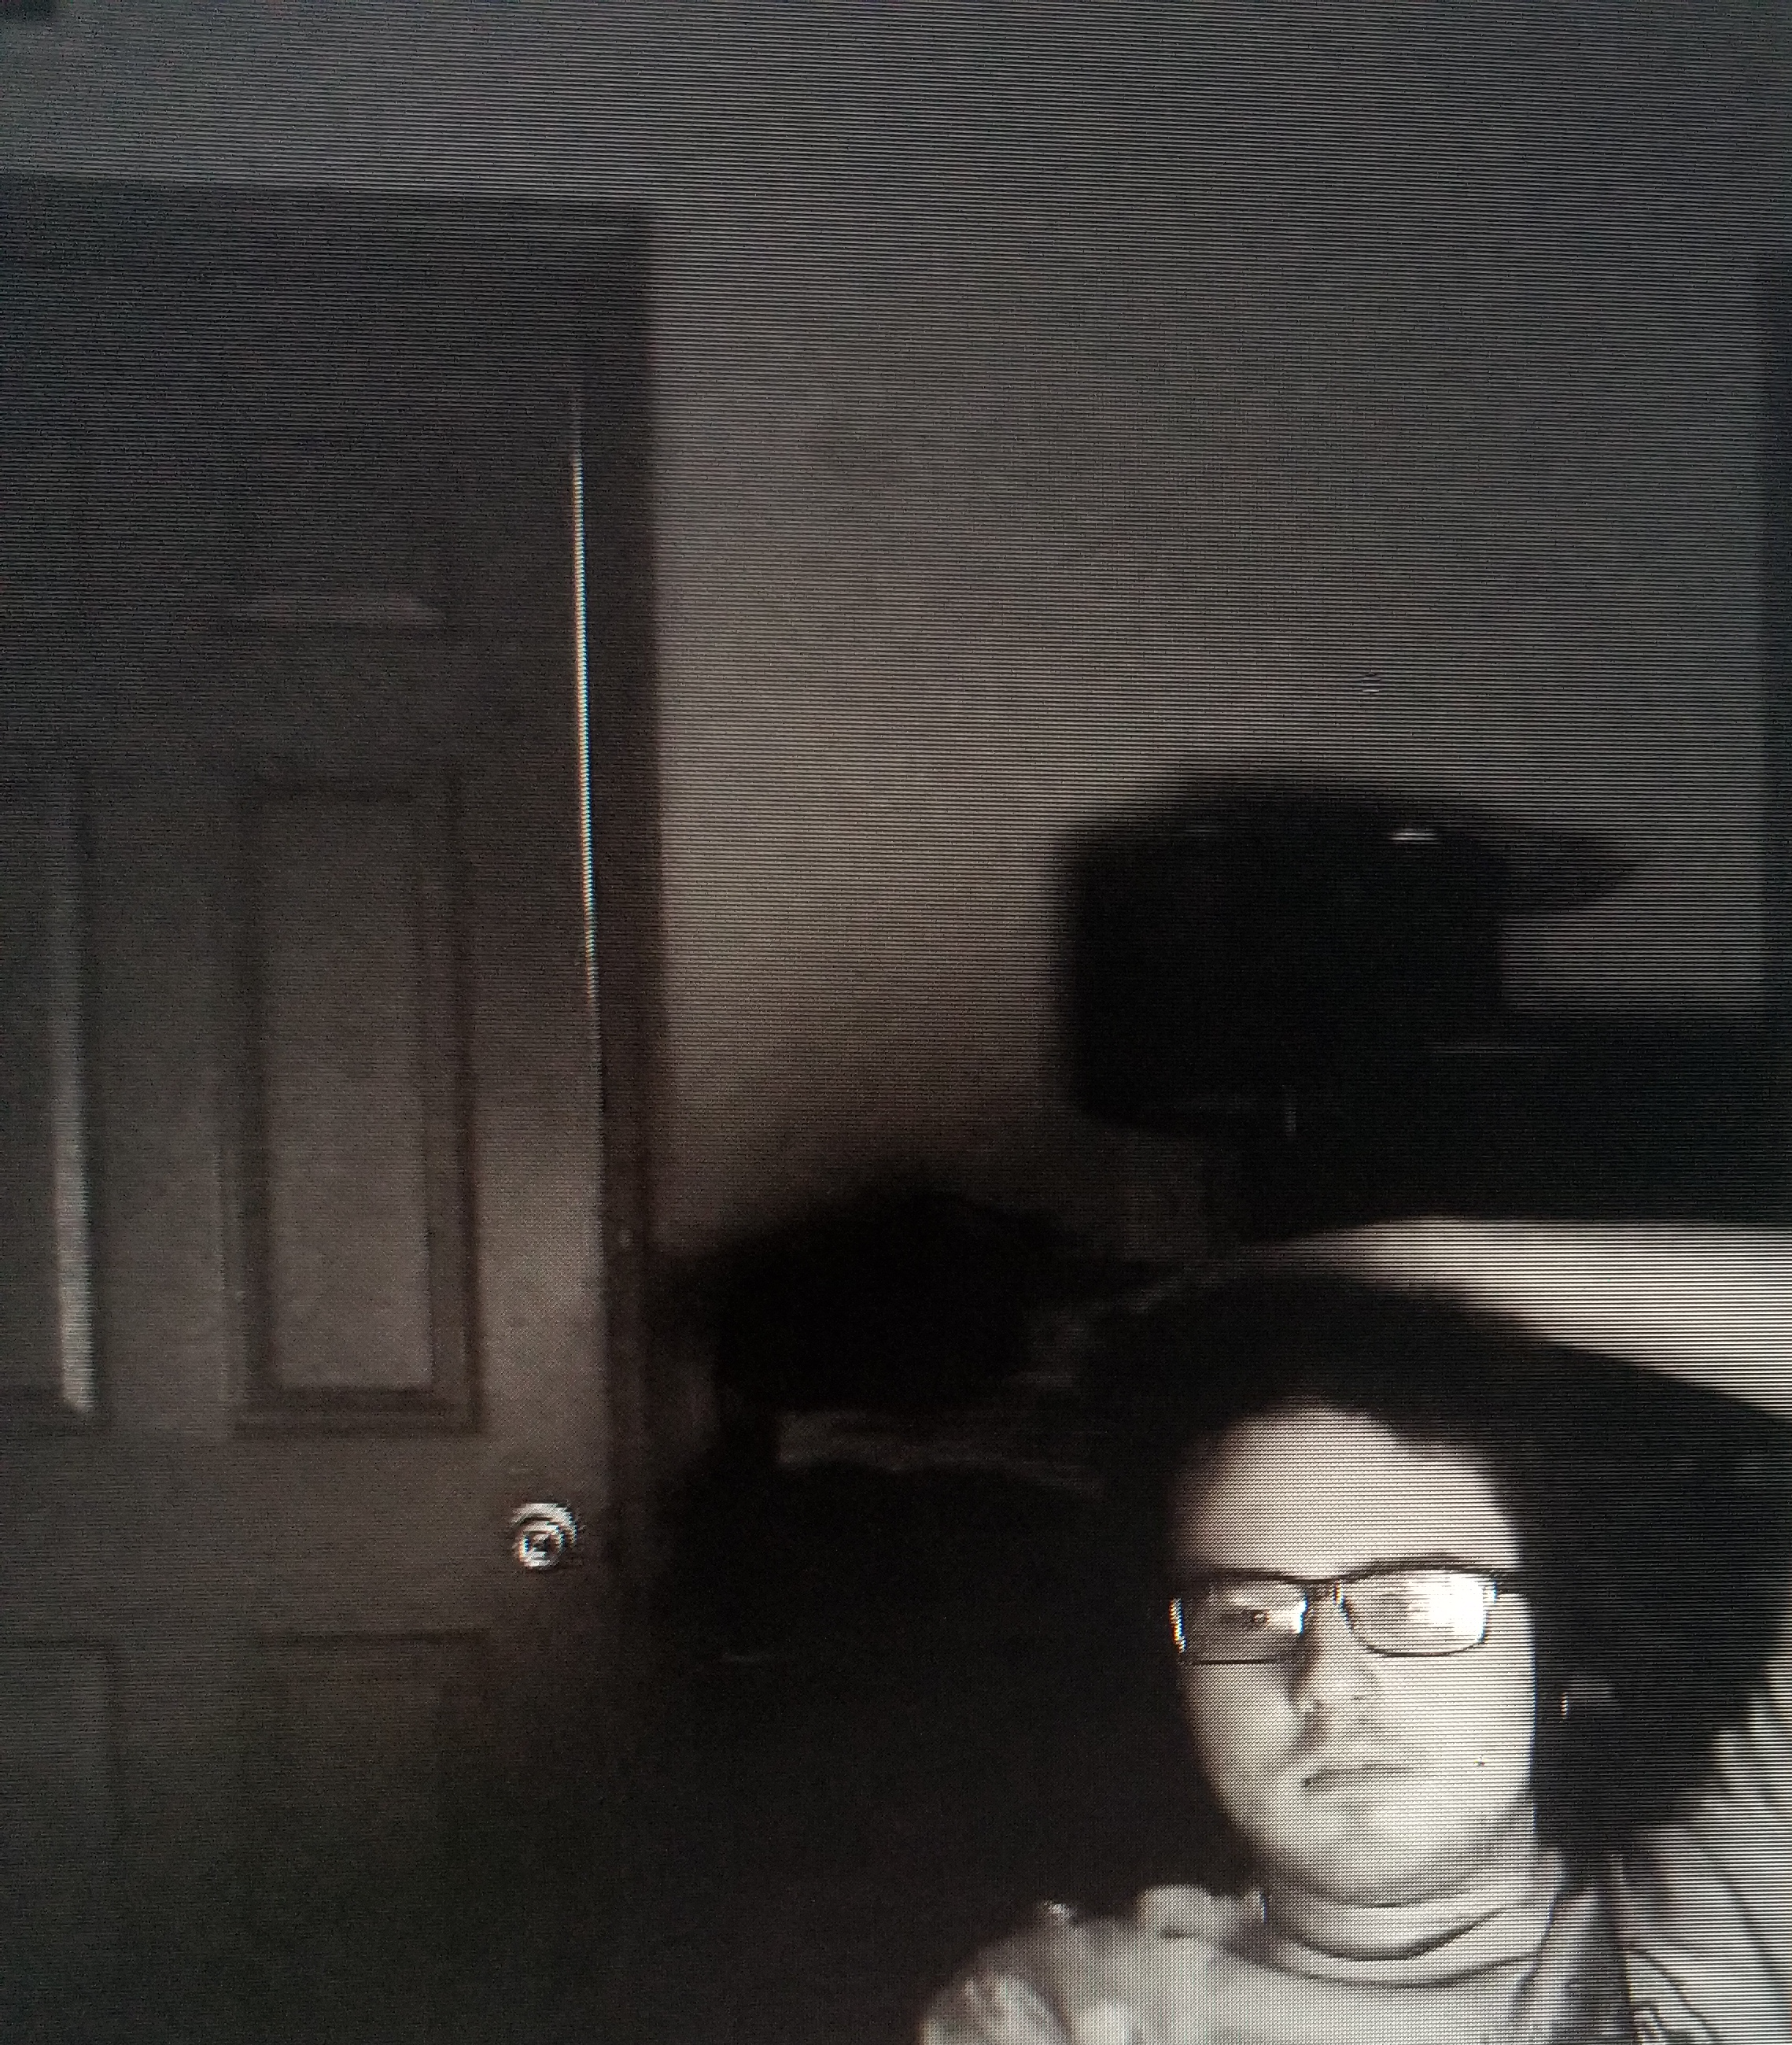
\includegraphics[width=\linewidth]{lackOfMotionCropped.png}
    \caption{Lack Of Motion}
    \label{fig:Performance of Original Pencil Drawing Program}
\end{figure}

\begin{figure}[h!]
    \includegraphics[width=\linewidth]{slightMotionCropped.jpg}
    \caption{Slight Motion}
    \label{fig:Performance of Original Pencil Drawing Program}
\end{figure}

\subsection{Results}
Our initial expectation was that, as it had in our grayscaling experiment, the GPU's performance relative to the CPU would rise as its task became larger and more complex. In addition, we believed that working with videos rather than images would boost complexity enough that the GPU would be the more efficient test from the beginning, although this was far from certain as the CPU showed eight times the GPU's performance even with the most complex image.\\
This was once again only partially true. As with the prior experiment, the GPU was vastly slower than the CPU, taking over half a second at tasks the CPU could complete in under two centiseconds. The CPU's processing time was generally thirty times faster than the GPU's. This means that our initial belief that video processing would be complex enough for the GPU to overcome the CPU was incorrect.\\ 
However, where an increase in object speed (and therefore complexity) would lead to a 2.5\%-7.5\% increase in processing time for the CPU, it led to less than a 1.5\% increase for all GPU tests. Meanwhile, the average processing time increase for the CPU was almost eight times larger than its GPU counterpart.This indicates that, given a sufficiently complex video and a Raspberry Pi that could handle said complexity, the GPU would once again eventually outpace the CPU. This further proves the trend found in both our prior experiment and in Liu's pencil drawing experiment.\\
As with the prior experiment, our results can be found in figures 8 and 9 below. The trials refer to the object moved, while the speeds refer to the average for all objects. Additionally, our raw data can also be found below.\\

\begin{multicols}{2}
\begin{alltt}
{\footnotesize \input{cpuInterval0ArmFast.txt}}
{\footnotesize \input{gpuInterval1ArmFast.txt}}
\end{alltt}
\end{multicols}

\begin{figure}[h!]
    \includegraphics[width=\linewidth]{CPU and GPU Average Processing Time in Seconds.png}
    \caption{Average CPU and GPU processing time}
    \label{fig:Performance of Original Pencil Drawing Program}
\end{figure}
\begin{figure}[h!]
    \includegraphics[width=\linewidth]{Processing Time Increase By Trial.png}
    \caption{Percent increase in processing time for each trial}
    \label{fig:Performance of Original Pencil Drawing Program}
\end{figure}

\section{Conclusions and Future Work}
In conclusion, we found that sufficiently small tasks led to the Raspberry Pi's CPU heavily outpacing the GPU in terms of speed, with the gap between the two increasing as tasks grew smaller. While this differed from previous works, it is easily explained by differences in hardware. The Raspberry Pi is a relatively weak and simple computer, and its capabilities are not comparable to many of the devices tested in similar experiments. This is further backed by an instance of our experiments agreeing with their predecessors, this being the existence of a trend in which the GPU's performance relative to the CPU steadily increases with larger and more complex tasks. According to the trend, had technical issues not prevented larger tasks from being tested, the RPi GPU's performance would have eventually outpaced that of the RPi CPU. This trend is clearly present in our experiments. Both show that when complexity is increased, the GPU takes relatively less additional time to handle that complexity. Since the CPU's processing time rose at a higher rate than the GPU's, it logically follows that the CPU's processing time will eventually meet and surpass that of the GPU with a sufficiently complex task.\\
There is plentiful area for more work on the subject in the future. As an example, one could determine how to overcome the crashing issue of our GPU-based grayscaling program. This would make it possible to verify that the GPU eventually overcomes the CPU's performance, as well as when this occurs. We have already had some successes in this area ourselves, though it has come with its own issues on the side. Additionally, one could compare both various models of Pi and various GPUs in general. Our own experiment was limited by using specifically the CPU and GPU of the Canakit RPi3, which we believe was likely a major reason for the GPU falling behind. A broader test of various CPUs and GPUs could provide a better picture of how various models of each compare.\\
Similarly, our second experiment also leaves plenty of room to be expanded. Like the pencil drawing experiment, it was heavily limited by the hardware of the RPi3. This forced us to take actions such as grayscaling the image before working with it, which would not be necessary with more resourceful hardware. Future work on this side could include attempting the video processing experiment with color video. It could also investigate how a lower or higher luminosity threshold affects the efficiency of the CPU and GPU, compared to our threshold set solely at 70. Additionally, it too could be tested with a broader set of hardware.



%Parallel Fast Pencil Drawing Generation Algorithm Based on GPU \cite{Liu}. \\
%Video Anomaly Detection in Real Time on a Power-Aware Heterogeneous Platform \cite{Blair}.
\newpage
\bibliography{references.bib}
\bibliographystyle{ieeetr}

\end{document}
